%==============================================================
%  EE201 -- Circuit Theory I
%  Lecture 10 : LTI Resistive Circuits and Equivalent One-Ports
%  M. Mert Ankaralı, METU EEE
%
%  Compile:  ./build.sh      (or: pdflatex EE201_Lecture_10.tex, twice)
%==============================================================
\documentclass[11pt,a4paper]{article}

%-------------------- packages --------------------------------
\usepackage[T1]{fontenc}
\usepackage[utf8]{inputenc}
\usepackage[english]{babel}
\usepackage{lmodern}
\usepackage[margin=2.3cm,top=2.0cm,bottom=1.9cm,headheight=14pt,headsep=9pt]{geometry}
\usepackage{amsmath,amssymb}
\usepackage{array,booktabs,tabularx}
\usepackage{enumitem}
\usepackage[table]{xcolor}
\usepackage{fancyhdr}
\usepackage{titlesec}
\usepackage{graphicx}
\usepackage[most]{tcolorbox}
\usepackage{tikz}
\usepackage[american,siunitx]{circuitikz}
\usetikzlibrary{matrix,arrows.meta,positioning,calc,decorations.pathmorphing,decorations.pathreplacing,decorations.markings,patterns,shapes.geometric}
\usepackage[colorlinks=true,allcolors=metured,breaklinks=true]{hyperref}

%-------------------- colour system ---------------------------
% One colour per physical quantity, used identically in the slides.
\definecolor{metured}{RGB}{155,27,48}    % headings, structure
\definecolor{metugray}{RGB}{88,89,91}
\definecolor{ccur}{RGB}{0,102,170}       % CURRENT  -- blue
\definecolor{cvolt}{RGB}{214,120,0}      % VOLTAGE  -- orange
\definecolor{cpow}{RGB}{23,128,74}       % POWER / ENERGY -- green
\definecolor{ccharge}{RGB}{124,60,160}   % CHARGE   -- purple
\definecolor{cflux}{RGB}{0,138,138}      % FLUX -- teal
\definecolor{boxgray}{RGB}{245,245,245}
\definecolor{copper}{RGB}{184,98,30}

\newcommand{\Icol}[1]{\textcolor{ccur}{#1}}
\newcommand{\Vcol}[1]{\textcolor{cvolt}{#1}}
\newcommand{\Pcol}[1]{\textcolor{cpow}{#1}}
\newcommand{\Qcol}[1]{\textcolor{ccharge}{#1}}
\newcommand{\Fcol}[1]{\textcolor{cflux}{#1}}

%-------------------- units (no siunitx dependency) -----------
\newcommand{\uni}[1]{\,\mathrm{#1}}
\newcommand{\A}{\uni{A}}   \newcommand{\V}{\uni{V}}
\newcommand{\W}{\uni{W}}   \newcommand{\J}{\uni{J}}
\newcommand{\Cb}{\uni{C}}  \newcommand{\s}{\uni{s}}
\newcommand{\Sie}{\uni{S}} \newcommand{\Wb}{\uni{Wb}}

%-------------------- layout ----------------------------------
\pagestyle{fancy}
\fancyhf{}
\lhead{\small\textcolor{metugray}{EE201 -- Circuit Theory I}}
\rhead{\small\textcolor{metugray}{Lecture 10: LTI Resistive Circuits and Equivalent One-Ports}}
\cfoot{\small\thepage}
\renewcommand{\headrulewidth}{0.4pt}

\titleformat{\section}{\large\bfseries\color{metured}}{\thesection.}{0.6em}{}
\titleformat{\subsection}{\normalsize\bfseries\color{metugray}}{\thesubsection.}{0.6em}{}
\titlespacing*{\section}{0pt}{1.4ex plus .3ex}{0.7ex}
\titlespacing*{\subsection}{0pt}{1.1ex plus .2ex}{0.5ex}

\setlist[itemize]{itemsep=2pt,topsep=3pt,parsep=0pt,leftmargin=1.5em}
\setlist[enumerate]{itemsep=2pt,topsep=3pt,parsep=0pt,leftmargin=1.7em}
\setlength{\parindent}{0pt}
\setlength{\parskip}{0.7ex plus .1ex}
\raggedbottom
\widowpenalty=10000
\clubpenalty=10000
\brokenpenalty=10000

%-------------------- boxes -----------------------------------
\newtcolorbox{definitionbox}[1]{enhanced,
  colback=metured!4, colframe=metured, boxrule=0.9pt,
  fonttitle=\bfseries, title={#1}, arc=2pt,
  left=7pt,right=7pt,top=5pt,bottom=5pt, before skip=7pt, after skip=7pt,
  before upper={\setlength{\parskip}{0.6ex plus .1ex}}}

\newtcolorbox{ideabox}[1][Key idea]{enhanced,
  colback=ccur!5, colframe=ccur, boxrule=0.9pt,
  fonttitle=\bfseries, title={#1}, arc=2pt,
  left=7pt,right=7pt,top=5pt,bottom=5pt, before skip=7pt, after skip=7pt,
  before upper={\setlength{\parskip}{0.6ex plus .1ex}}}

\newtcolorbox{examplebox}[1][Example]{enhanced,
  colback=cpow!4, colframe=cpow, boxrule=0.9pt,
  fonttitle=\bfseries, title={#1}, arc=2pt,
  left=7pt,right=7pt,top=5pt,bottom=5pt, before skip=7pt, after skip=7pt,
  before upper={\setlength{\parskip}{0.6ex plus .1ex}}}

\newtcolorbox{cautionbox}[1][Careful]{enhanced,
  colback=cvolt!6, colframe=cvolt, boxrule=0.9pt,
  fonttitle=\bfseries, title={#1}, arc=2pt,
  left=7pt,right=7pt,top=5pt,bottom=5pt, before skip=7pt, after skip=7pt,
  before upper={\setlength{\parskip}{0.6ex plus .1ex}}}

%-------------------- circuitikz defaults ---------------------
\ctikzset{bipoles/length=0.9cm, color=black,
          label/align=straight,
          bipoles/generic/height=0.28, bipoles/generic/width=0.62}
\tikzset{
  iar/.style={-{Stealth[length=2.2mm]}, ccur, thick},
  pol/.style={font=\small, text=cvolt},
  glab/.style={font=\footnotesize, text=metured},
  ttl/.style={font=\scriptsize\bfseries, text=metugray},
  capn/.style={font=\scriptsize, text=metugray, align=center},
  bigarr/.style={-{Stealth[length=3mm]}, very thick, metugray},
  gnode/.style={circle, fill=metured, inner sep=0pt, minimum size=4.4pt},
  nlab/.style={circle, draw=metured, text=metured, font=\scriptsize, inner sep=0.7pt},
  blab/.style={font=\footnotesize, text=black!80},
  gbr/.style={black!75, thick, postaction={decorate, decoration={markings,
      mark=at position 0.56 with {\arrow{Stealth[length=2.5mm]}}}}},
  apbr/.style={ccur, line width=1.7pt, postaction={decorate, decoration={markings,
      mark=at position 0.56 with {\arrow{Stealth[length=2.8mm]}}}}},
  hal/.style={draw=cpow!60, line width=6pt, opacity=0.35, line cap=round, line join=round},
  elem/.style={draw=metugray, thick, fill=metulight},
}
\definecolor{metulight}{RGB}{243,240,241}

%-------------------- Lecture 10 circuit macros ---------------
\newcommand{\ohm}{\,\Omega}
%  Port terminals a (top) and b (bottom) at x = #1, with i (entering at a) and v
\newcommand{\portlabels}[1]{%
  \draw[fill=white] (#1,1.6) circle (1.8pt) node[above=1pt, font=\small] {$a$};
  \draw[fill=white] (#1,0.4) circle (1.8pt) node[below=1pt, font=\small] {$b$};
  \draw[iar] (#1-0.78,1.84) -- (#1-0.22,1.84);
  \node[font=\small, text=ccur] at (#1-0.5,2.12) {$i$};
  \node[pol] at (#1,1.28) {$+$}; \node[pol] at (#1,0.72) {$-$};
  \node[font=\small, text=cvolt] at (#1+0.3,1.0) {$v$};}
%  Two boxes joined at a port: #1 left name, #2 right name
\newcommand{\pairbox}[2]{%
  \draw[elem] (0,0) rectangle (1.7,2.0); \node at (0.85,1.0) {#1};
  \draw[elem] (3.5,0) rectangle (5.2,2.0); \node at (4.35,1.0) {#2};
  \draw (1.7,1.6) -- (3.5,1.6); \draw (1.7,0.4) -- (3.5,0.4);
  \portlabels{2.6}}
%  Substitution: N2 replaced by a voltage source (#1 = 0) or a current source (#1 = 1)
\newcommand{\subsbox}[1]{%
  \draw[elem] (0,0) rectangle (1.7,2.0); \node at (0.85,1.0) {$N_1$};
  \draw (1.7,1.6) -- (3.6,1.6); \draw (1.7,0.4) -- (3.6,0.4);
  \ifcase#1
    \draw (3.6,0.4) to[american voltage source, invert] (3.6,1.6);
    \node[font=\small, right] at (3.95,1.0) {$\Vcol{v_s} = \Vcol{v}$};
  \or
    \draw (3.6,1.6) to[american current source] (3.6,0.4);
    \node[font=\small, right] at (3.95,1.0) {$\Icol{i_s} = \Icol{i}$};
  \fi
  \portlabels{2.6}}
%  A one-port N seen from its terminals
\newcommand{\oneport}[1]{%
  \draw[elem] (1.3,0) rectangle (2.9,2.0); \node at (2.1,1.0) {#1};
  \draw (0,1.6) -- (1.3,1.6); \draw (0,0.4) -- (1.3,0.4);
  \draw[fill=white] (0,1.6) circle (1.8pt) node[left=1pt, font=\small] {$a$};
  \draw[fill=white] (0,0.4) circle (1.8pt) node[left=1pt, font=\small] {$b$};
  \draw[iar] (0.3,1.84) -- (0.95,1.84); \node[font=\small, text=ccur] at (0.62,2.12) {$i$};
  \draw[iar] (0.95,0.16) -- (0.3,0.16); \node[font=\small, text=ccur] at (0.62,-0.13) {$i$};
  \node[pol] at (0.3,1.28) {$+$}; \node[pol] at (0.3,0.72) {$-$};
  \node[font=\small, text=cvolt] at (0.65,1.0) {$v$};}
%  Terminals a, b at (#1,#2) and (#1,0); labels on side #3 (left/right)
\newcommand{\abterm}[3]{%
  \draw[fill=white] (#1,#2) circle (1.8pt) node[#3=1pt, font=\small] {$a$};
  \draw[fill=white] (#1,0) circle (1.8pt) node[#3=1pt, font=\small] {$b$};}
%  k resistors in series between a and b
\newcommand{\seriesR}{%
  \draw (0,1.2) to[R, l=$R_1$] (1.3,1.2) to[R, l=$R_2$] (2.6,1.2) -- (2.8,1.2);
  \node at (3.15,1.2) {$\cdots$};
  \draw (3.5,1.2) -- (3.7,1.2) to[R, l=$R_k$] (5.0,1.2) -- (5.0,0) -- (0,0);
  \abterm{0}{1.2}{left}}
%  k voltage sources in series between a and b (+ towards a)
\newcommand{\seriesV}{%
  \draw (0,1.2) to[american voltage source, l=$v_{s1}$] (1.3,1.2)
        to[american voltage source, l=$v_{s2}$] (2.6,1.2) -- (2.8,1.2);
  \node at (3.15,1.2) {$\cdots$};
  \draw (3.5,1.2) -- (3.7,1.2) to[american voltage source, l=$v_{sk}$] (5.0,1.2)
        -- (5.0,0) -- (0,0);
  \abterm{0}{1.2}{left}}
%  k resistors in parallel between a and b
\newcommand{\parR}{%
  \draw (0,1.5) -- (4.2,1.5); \draw (0,0) -- (4.2,0);
  \draw (0.8,1.5) to[R, l=$R_1$] (0.8,0);
  \draw (2.0,1.5) to[R, l=$R_2$] (2.0,0);
  \node at (3.25,0.75) {$\cdots$};
  \draw (4.2,1.5) to[R, l=$R_k$] (4.2,0);
  \abterm{0}{1.5}{left}}
%  k current sources in parallel between a and b (arrows towards a)
\newcommand{\parI}{%
  \draw (0,1.5) -- (4.2,1.5); \draw (0,0) -- (4.2,0);
  \draw (0.8,0) to[american current source, l_=$i_{s1}$] (0.8,1.5);
  \draw (2.0,0) to[american current source, l_=$i_{s2}$] (2.0,1.5);
  \node at (3.25,0.75) {$\cdots$};
  \draw (4.2,0) to[american current source, l_=$i_{sk}$] (4.2,1.5);
  \abterm{0}{1.5}{left}}
%  One equivalent element between a (height #1) and b; #2: circuitikz options
\newcommand{\eqone}[2]{%
  \draw (0,#1) -- (1.0,#1) to[#2] (1.0,0) -- (0,0);
  \abterm{0}{#1}{left}}
%  Voltage source v_s (#1) in series with R (#2), terminals on the right
\newcommand{\vsR}[2]{%
  \draw (0,0) to[american voltage source, invert, l=#1] (0,1.8);
  \draw (0,1.8) to[R, l=#2] (1.7,1.8) -- (2.4,1.8);
  \draw (0,0) -- (2.4,0);
  \abterm{2.4}{1.8}{right}}
%  Current source i_s (#1) in parallel with R (#2), terminals on the right
\newcommand{\isR}[2]{%
  \draw (0,0) to[american current source, l=#1] (0,1.8);
  \draw (0,1.8) -- (2.4,1.8); \draw (0,0) -- (2.4,0);
  \draw (1.2,1.8) to[R, l=#2] (1.2,0);
  \abterm{2.4}{1.8}{right}}
%  Port current i entering at a and port voltage v, for \vsR / \isR
\newcommand{\stport}{%
  \draw[iar] (2.25,2.07) -- (1.85,2.07); \node[font=\small, text=ccur] at (2.05,2.35) {$i$};
  \node[pol] at (2.45,1.35) {$+$}; \node[pol] at (2.45,0.45) {$-$};
  \node[font=\small, text=cvolt] at (2.75,0.9) {$v$};}
%  The example circuit: 12 V, 2 ohm, 6 ohm in N1; at the port:
%  #1 = 0: 3 ohm, 1: 6 V source, 2: 2 A source
\newcommand{\exN}[1]{%
  \draw[dashed, metugray, rounded corners=3pt] (-0.95,-0.4) rectangle (2.55,2.5);
  \node[font=\small, text=metugray, anchor=south west, inner sep=1pt] at (-0.95,2.52) {$N_1$};
  \draw (0,0) to[american voltage source, invert, l=$12\V$] (0,2);
  \draw (0,2) to[R, l=$2\ohm$] (2.0,2) -- (3.6,2);
  \draw (2.0,2) to[R, l_=$6\ohm$] (2.0,0);
  \draw (0,0) -- (3.6,0);
  \ifcase#1
    \draw (3.6,2) to[R, l=$3\ohm$] (3.6,0);
  \or
    \draw (3.6,0) to[american voltage source, invert, l_=$6\V$] (3.6,2);
  \or
    \draw (3.6,2) to[american current source, l=$2\A$] (3.6,0);
  \fi
  \draw[fill=white] (2.85,2) circle (1.8pt) node[above=1pt, font=\small] {$a$};
  \draw[fill=white] (2.85,0) circle (1.8pt) node[below=1pt, font=\small] {$b$};}
%  Small classification circuits: source #1 and element #2 (circuitikz options)
\newcommand{\mini}[2]{%
  \draw (0,0) to[#1] (0,1.5) -- (1.4,1.5) to[#2] (1.4,0) -- (0,0);}

\begin{document}

%-------------------- title block -----------------------------
\begin{center}
\begin{tcolorbox}[enhanced, colback=metured!5, colframe=metured, boxrule=1pt,
                  arc=3pt, left=10pt,right=10pt,top=7pt,bottom=7pt, width=\textwidth]
\begin{center}
  {\small\scshape Middle East Technical University}\\[2pt]
  {\small\scshape Department of Electrical and Electronics Engineering}\\[7pt]
  {\Large\bfseries\color{metured} EE201 -- Circuit Theory I}\\[4pt]
  {\large\bfseries Lecture 10: LTI Resistive Circuits and Equivalent One-Ports}\\[6pt]
  {\small M. Mert Ankaralı}
\end{center}
\end{tcolorbox}
\end{center}
\vspace{-0.5em}

\begin{center}
\small
\begin{tabular}{@{}l l@{}}
\toprule
\multicolumn{2}{@{}l}{\textbf{Colour code used in these notes and in the slides}}\\
\midrule
\Icol{$\blacksquare$}~current $i$ \quad \Vcol{$\blacksquare$}~voltage $v$ &
\textcolor{metugray}{$\blacksquare$}~a part of a circuit (box $N$), terminals $a$, $b$\\
\bottomrule
\end{tabular}
\end{center}

\textbf{Why this lecture?} So far, KCL and KVL were written for any circuit, with any
elements. From now on we restrict the elements. In an \textbf{LTI resistive circuit} every
equation is linear and algebraic, so the circuit can be simplified before it is solved. This
lecture gives the tools for that: the substitution theorem, one-ports and their equivalents,
series and parallel connections, and the exchange of a voltage source and a current source.

%==============================================================
\section{LTI resistive circuits}

Three pairs of words describe a circuit. Each pair is defined by what the circuit contains.

\begin{definitionbox}{Nonlinear, time-varying, dynamic}
\begin{itemize}
  \item A \textbf{nonlinear} circuit contains a nonlinear resistor, inductor, capacitor or
        dependent source. A circuit is \textbf{linear} if it is not nonlinear.
  \item A \textbf{time-varying} circuit contains a time-varying resistor, inductor, capacitor
        or dependent source. A circuit is \textbf{time-invariant} if it is not time-varying.
  \item A \textbf{dynamic} circuit contains an inductor or a capacitor. A circuit is
        \textbf{resistive} if it is not dynamic.
\end{itemize}
An \textbf{LTI resistive circuit} is linear, time-invariant and resistive. It contains only
LTI resistors, linear time-invariant dependent sources and independent sources.
\end{definitionbox}

\begin{cautionbox}[Independent sources do not count]
The lists above do not mention independent sources. A source $\Vcol{v_s(t)} = 10\cos t\V$
driving an LTI resistor gives an LTI resistive circuit. The words describe the circuit, not the
waveform that drives it.
\end{cautionbox}

\textbf{What we gain.} In an LTI resistive circuit KCL and KVL are linear, and every element
equation is linear and algebraic: $v = Ri$ for a resistor, $v = \mu v_x$ or $i = g\,v_x$
for a dependent source. No derivative appears. Time enters only through the values of the
independent sources, so at each instant the circuit is solved like a circuit with constant
sources.

\begin{examplebox}[Example 10.1 --- which circuit is which?]
Each circuit is a source and one more element.
\begin{center}
\small
\begin{tabular}{@{}c@{\hspace{2mm}}c@{\hspace{2mm}}c@{\hspace{2mm}}c@{\hspace{2mm}}c@{}}
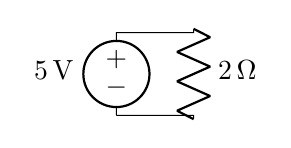
\begin{tikzpicture}[scale=0.7]
  \mini{american voltage source, invert, l=$5\V$}{R, l=$2\ohm$}
\end{tikzpicture} &
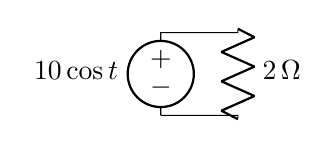
\begin{tikzpicture}[scale=0.7]
  \mini{american voltage source, invert, l=$10\cos t$}{R, l=$2\ohm$}
\end{tikzpicture} &
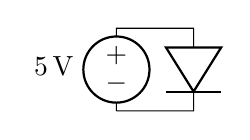
\begin{tikzpicture}[scale=0.7]
  \mini{american voltage source, invert, l=$5\V$}{D}
\end{tikzpicture} &
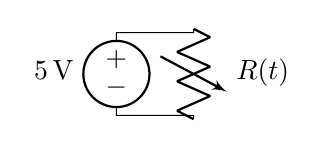
\begin{tikzpicture}[scale=0.7]
  \mini{american voltage source, invert, l=$5\V$}{vR, l=$R(t)$}
\end{tikzpicture} &
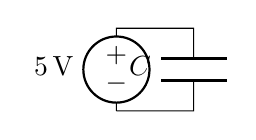
\begin{tikzpicture}[scale=0.7]
  \mini{american voltage source, invert, l=$5\V$}{C, l_=$C$}
\end{tikzpicture}\\
(a) LTI resistive & (b) LTI resistive & (c) nonlinear (diode) & (d) time-varying & (e) dynamic
\end{tabular}
\end{center}
(b) is LTI resistive although its source varies in time. In (d), $R(t) = 2 + \sin t\ \Omega$.
(c) and (d) are still resistive; (e) is still linear and time-invariant.
\end{examplebox}

%==============================================================
\section{The substitution theorem}

Split a circuit into two parts $N_1$ and $N_2$, joined at two terminals $a$ and $b$. Let
$\Vcol{v(t)}$ be the voltage between $a$ and $b$, and $\Icol{i(t)}$ the current from $N_1$
into $N_2$ at $a$.

\begin{center}
\begin{tabular}{@{}c@{\hspace{6mm}}c@{\hspace{6mm}}c@{}}
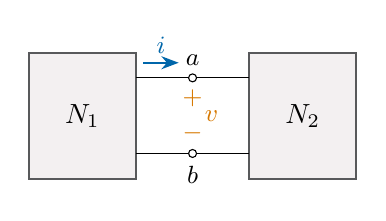
\begin{tikzpicture}[scale=0.8]
  \pairbox{$N_1$}{$N_2$}
\end{tikzpicture} &
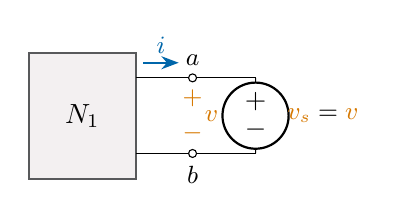
\begin{tikzpicture}[scale=0.8]
  \subsbox{0}
\end{tikzpicture} &
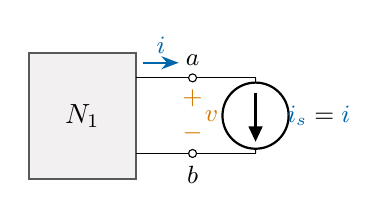
\begin{tikzpicture}[scale=0.8]
  \subsbox{1}
\end{tikzpicture}\\[2pt]
{\small (I) the circuit} & {\small (II) $N_2$ $\to$ voltage source}
  & {\small (III) $N_2$ $\to$ current source}
\end{tabular}
\end{center}

\begin{ideabox}[Substitution theorem]
Replace $N_2$ by an independent voltage source $\Vcol{v_s(t)} = \Vcol{v(t)}$, or by an
independent current source $\Icol{i_s(t)} = \Icol{i(t)}$. No branch voltage or branch current
inside $N_1$ changes. An observer inside $N_1$ cannot tell (I), (II) and (III) apart.
\end{ideabox}

\textbf{Why it works.} The equations inside $N_1$ (its KCL, KVL and element equations) do
not change. $N_1$ meets the rest of the circuit only through $\Vcol{v}$ and $\Icol{i}$. The
source fixes one of them at the value it had in (I), and the solution of (I) still satisfies
every equation of (II) and (III). $N_2$ can be anything, even nonlinear: only its port values
matter.

\textbf{One condition.} The new circuit must have a unique solution. If $N_1$ is a single
current source, replacing $N_2$ by a current source puts two current sources in series: their
currents are equal, but the voltage $\Vcol{v}$ is no longer fixed.

\begin{examplebox}[Example 10.2 --- substitution in a small circuit]
\begin{center}
\begin{tabular}{@{}c@{\hspace{3mm}}c@{\hspace{3mm}}c@{}}
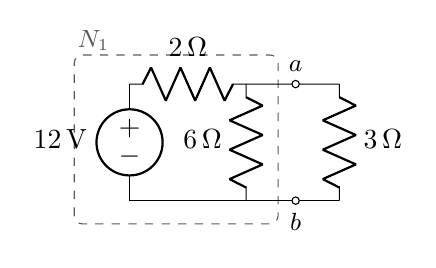
\begin{tikzpicture}[scale=0.74]
  \exN{0}
\end{tikzpicture} &
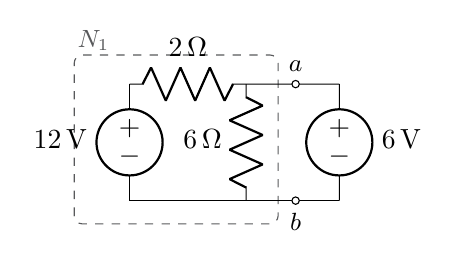
\begin{tikzpicture}[scale=0.74]
  \exN{1}
\end{tikzpicture} &
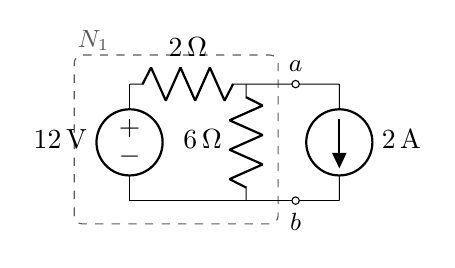
\begin{tikzpicture}[scale=0.74]
  \exN{2}
\end{tikzpicture}\\[2pt]
{\small (I) $N_2$: the $3\ohm$ resistor} & {\small (II) a $6\V$ source} & {\small (III) a $2\A$ source}
\end{tabular}
\end{center}
\textbf{(I)} The $6\ohm$ and $3\ohm$ are in parallel: $2\ohm$. The two $2\ohm$ share the
$12\V$, so $\Vcol{v} = 6\V$, and $\Icol{i} = 6/3 = 2\A$ flows into $N_2$. Inside $N_1$: the
$2\ohm$ carries $(12 - 6)/2 = 3\A$ and the $6\ohm$ carries $6/6 = 1\A$.

\textbf{(II)} The $6\V$ source fixes $\Vcol{v} = 6\V$. Again the $2\ohm$ carries $3\A$ and the
$6\ohm$ carries $1\A$; the source takes the remaining $2\A$.

\textbf{(III)} The $2\A$ source takes $2\A$ from node $a$. KCL at $a$:
$(12 - \Vcol{v})/2 = \Vcol{v}/6 + 2$, so $\Vcol{v} = 6\V$, and the currents inside $N_1$ are
$3\A$ and $1\A$ again.
\end{examplebox}

The theorem lets us cut a circuit and study one part at a time. It is also the key step in
later proofs, where a complicated part is replaced by a source.

%==============================================================
\section{Ports and equivalent one-ports}

\begin{definitionbox}{Port, one-port}
A pair of terminals is a \textbf{port} if the current entering one terminal equals the current
leaving the other. A \textbf{one-port} is a circuit, or a circuit element, with one pair of
terminals accessible from outside.
\end{definitionbox}

\begin{center}
\begin{minipage}[c]{0.3\linewidth}
\centering
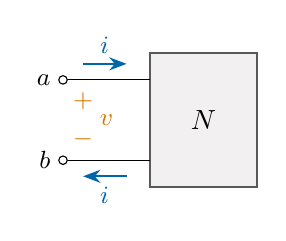
\begin{tikzpicture}[scale=0.85]
  \oneport{$N$}
\end{tikzpicture}
\end{minipage}%
\hfill
\begin{minipage}[c]{0.66\linewidth}
A one-port is always a port: by KCL on a closed surface around $N$, the current $\Icol{i}$
that enters at $a$ leaves at $b$. We take $\Icol{i}$ entering the $+$ terminal of
$\Vcol{v}$. The relation between $\Vcol{v}$ and $\Icol{i}$ is the \textbf{$i$--$v$
characteristic} of the one-port. A resistor is the simplest one-port: $\Vcol{v} = R\Icol{i}$.
\end{minipage}
\end{center}

\begin{definitionbox}{Equivalent one-ports}
Two one-ports $N_1$ and $N_2$ are \textbf{equivalent}, $N_1 \equiv N_2$, if they have the
same $i$--$v$ characteristic at their terminals. Then, for any one-port $N_0$ connected to
them, every branch voltage and branch current inside $N_0$ is the same with $N_1$ or with
$N_2$.
\end{definitionbox}

\begin{center}
\begin{tabular}{@{}c@{\hspace{10mm}}c@{}}
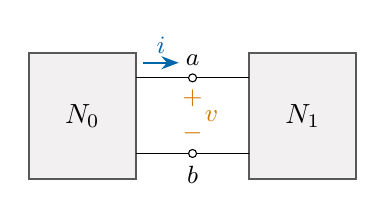
\begin{tikzpicture}[scale=0.8]
  \pairbox{$N_0$}{$N_1$}
\end{tikzpicture} &
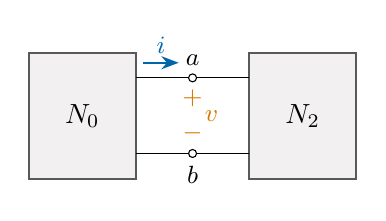
\begin{tikzpicture}[scale=0.8]
  \pairbox{$N_0$}{$N_2$}
\end{tikzpicture}
\end{tabular}
\end{center}
$N_0$ meets the rest only through $\Vcol{v}$ and $\Icol{i}$. The equations of the whole
circuit are those of $N_0$ plus the $i$--$v$ characteristic at the port. Equivalent one-ports
give the same equations, so the same solution inside $N_0$. Inside $N_1$ and $N_2$ the
branch values may differ.

%==============================================================
\section{Series and parallel connections}

\subsection*{Series connection}
In a series connection the same current $\Icol{i}$ flows through every element (KCL), and
the voltages add (KVL).

\begin{center}
\begin{tabular}{@{}c@{\hspace{2mm}}c@{\hspace{2mm}}c@{\hspace{4mm}}l@{}}
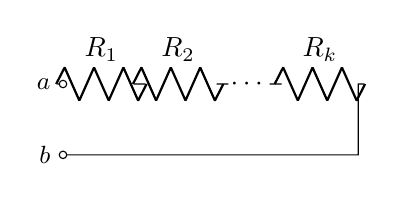
\begin{tikzpicture}[scale=0.75, baseline=(c.base)]
  \seriesR \coordinate (c) at (0,0.5);
\end{tikzpicture} & $\equiv$ &
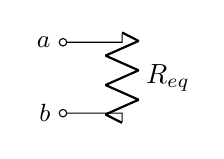
\begin{tikzpicture}[scale=0.75, baseline=(c.base)]
  \eqone{1.2}{R, l=$R_{eq}$} \coordinate (c) at (0,0.5);
\end{tikzpicture} &
$R_{eq} = R_1 + R_2 + \dots + R_k$\\[10pt]
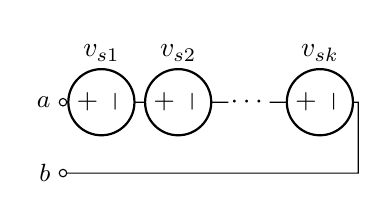
\begin{tikzpicture}[scale=0.75, baseline=(c.base)]
  \seriesV \coordinate (c) at (0,0.5);
\end{tikzpicture} & $\equiv$ &
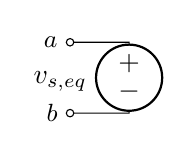
\begin{tikzpicture}[scale=0.75, baseline=(c.base)]
  \eqone{1.2}{american voltage source, l_=$v_{s,eq}$} \coordinate (c) at (0,0.5);
\end{tikzpicture} &
$v_{s,eq} = v_{s1} + v_{s2} + \dots + v_{sk}$
\end{tabular}
\end{center}
For the resistors: $\Vcol{v} = R_1\Icol{i} + \dots + R_k\Icol{i} = R_{eq}\Icol{i}$. The share
of $R_j$ is $\Vcol{v_j} = (R_j/R_{eq})\,\Vcol{v}$ (\textbf{voltage divider}). For the sources
all $+$ signs point towards $a$; a source turned the other way enters the sum with $-$.

\subsection*{Parallel connection}
In a parallel connection every element has the same voltage $\Vcol{v}$ (KVL), and the
currents add (KCL).

\begin{center}
\begin{tabular}{@{}c@{\hspace{2mm}}c@{\hspace{2mm}}c@{\hspace{4mm}}l@{}}
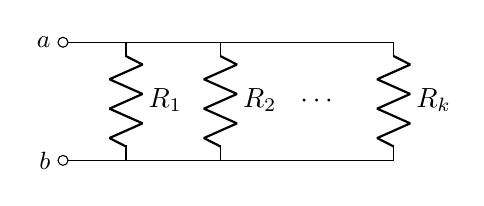
\begin{tikzpicture}[scale=1.0, baseline=(c.base)]
  \parR \coordinate (c) at (0,0.65);
\end{tikzpicture} & $\equiv$ &
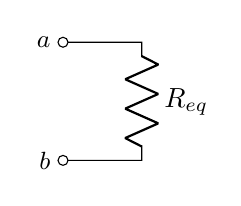
\begin{tikzpicture}[scale=1.0, baseline=(c.base)]
  \eqone{1.5}{R, l=$R_{eq}$} \coordinate (c) at (0,0.65);
\end{tikzpicture} &
$\dfrac{1}{R_{eq}} = \dfrac{1}{R_1} + \dfrac{1}{R_2} + \dots + \dfrac{1}{R_k}$\\[18pt]
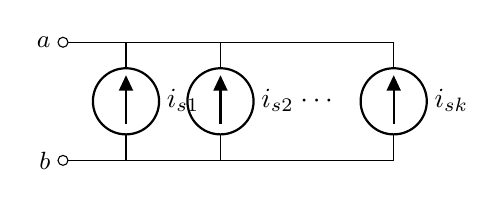
\begin{tikzpicture}[scale=1.0, baseline=(c.base)]
  \parI \coordinate (c) at (0,0.65);
\end{tikzpicture} & $\equiv$ &
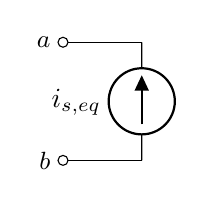
\begin{tikzpicture}[scale=1.0, baseline=(c.base)]
  \draw (1.0,0) to[american current source, l=$i_{s,eq}$] (1.0,1.5);
  \draw (0,1.5) -- (1.0,1.5); \draw (0,0) -- (1.0,0); \abterm{0}{1.5}{left}
  \coordinate (c) at (0,0.65);
\end{tikzpicture} &
$i_{s,eq} = i_{s1} + i_{s2} + \dots + i_{sk}$
\end{tabular}
\end{center}
With conductances $G_j = 1/R_j$: $\Icol{i} = G_1\Vcol{v} + \dots + G_k\Vcol{v} =
G_{eq}\Vcol{v}$, so $G_{eq} = G_1 + \dots + G_k$. The share of $R_j$ is
$\Icol{i_j} = (G_j/G_{eq})\,\Icol{i}$ (\textbf{current divider}). Two resistors:
$R_{eq} = R_1R_2/(R_1 + R_2)$.

\begin{cautionbox}[Two connections that are not allowed]
Two voltage sources with $v_{s1} \ne v_{s2}$ in parallel break KVL. Two current sources with
$i_{s1} \ne i_{s2}$ in series break KCL. With equal values the connection is allowed, but the
current shared by the two voltage sources (or the voltage shared by the two current sources)
is not fixed.
\end{cautionbox}

%==============================================================
\section{One source and one resistor}

Take a voltage source with a series resistor, and a current source with a parallel resistor.
In both, $\Icol{i}$ enters at $a$.

\begin{center}
\begin{tabular}{@{}c@{\hspace{14mm}}c@{}}
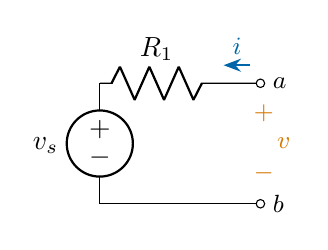
\begin{tikzpicture}[scale=0.85]
  \vsR{$v_s$}{$R_1$} \stport
\end{tikzpicture} &
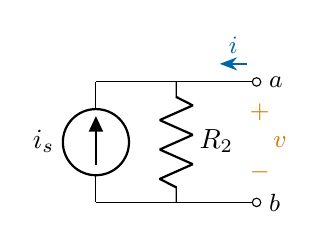
\begin{tikzpicture}[scale=0.85]
  \isR{$i_s$}{$R_2$} \stport
\end{tikzpicture}\\[2pt]
$\Vcol{v} = R_1\Icol{i} + v_s \qquad (1)$ &
$\Vcol{v} = R_2(\Icol{i} + i_s) = R_2\Icol{i} + R_2 i_s \qquad (2)$
\end{tabular}
\end{center}
In (2), $\Icol{i}$ and $i_s$ both flow into the top node, so $R_2$ carries $\Icol{i} + i_s$.
Both characteristics are straight lines in the $i$--$v$ plane. They are the same line when the
slopes and the intercepts agree.

\begin{center}
\begin{minipage}[c]{0.5\linewidth}
\begin{ideabox}[Source transformation]
The two one-ports are equivalent if
\[
  R_1 = R_2 = R \qquad\text{and}\qquad v_s = R\, i_s .
\]
Open circuit ($\Icol{i} = 0$): $\Vcol{v} = v_s$. Short circuit ($\Vcol{v} = 0$):
$\Icol{i} = -i_s$.
\end{ideabox}
\end{minipage}%
\hfill
\begin{minipage}[c]{0.45\linewidth}
\centering
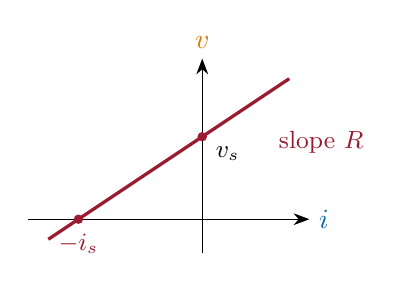
\begin{tikzpicture}[scale=0.85]
  \draw[-{Stealth[length=2mm]}] (-2.6,0) -- (1.6,0) node[right] {$\Icol{i}$};
  \draw[-{Stealth[length=2mm]}] (0,-0.5) -- (0,2.4) node[above] {$\Vcol{v}$};
  \draw[metured, very thick] (-2.3,-0.3) -- (1.3,2.1);
  \fill[metured] (0,1.233) circle (2pt); \node[font=\small] at (0.38,0.98) {$v_s$};
  \fill[metured] (-1.85,0) circle (2pt) node[below=2pt, font=\small] {$-i_s$};
  \node[font=\small, text=metured, anchor=west] at (1.0,1.15) {slope $R$};
\end{tikzpicture}
\end{minipage}
\end{center}

\begin{examplebox}[Example 10.3 --- a source transformation]
\begin{center}
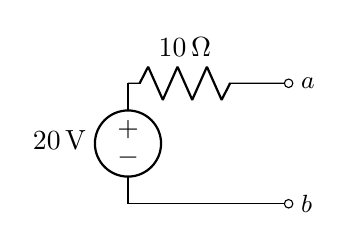
\begin{tikzpicture}[scale=0.85, baseline=(c.base)]
  \vsR{$20\V$}{$10\ohm$} \coordinate (c) at (0,0.8);
\end{tikzpicture}
\quad $\equiv$ \quad
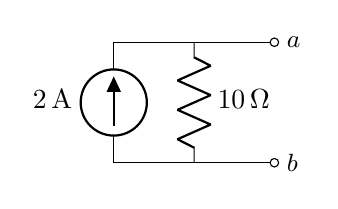
\begin{tikzpicture}[scale=0.85, baseline=(c.base)]
  \isR{$2\A$}{$10\ohm$} \coordinate (c) at (0,0.8);
\end{tikzpicture}
\end{center}
$R = 10\ohm$ and $i_s = v_s/R = 20/10 = 2\A$. Both have open-circuit voltage $20\V$ and
short-circuit current $2\A$ (out of $a$).
\end{examplebox}

\begin{examplebox}[Example 10.4 --- Example 10.2 again, by transformations]
Replace the $12\V$ source and the $2\ohm$ by a $6\A$ source in parallel with $2\ohm$. Now
$2\ohm$, $6\ohm$ and $3\ohm$ are in parallel: $G_{eq} = \tfrac12 + \tfrac16 + \tfrac13 =
1\Sie$, so $R_{eq} = 1\ohm$, and
\[
  \Vcol{v} = 6\A \times 1\ohm = 6\V, \qquad \Icol{i} = 6/3 = 2\A,
\]
as before. The part outside the transformed one-port sees the same $\Vcol{v}$ and
$\Icol{i}$. Inside it the values differ: the $12\V$ source carries $3\A$, while the $6\A$
source carries $6\A$.
\end{examplebox}

%==============================================================
\section{Solving LTI resistive circuits}

Series and parallel connections and source transformations simplify many circuits, but not
all. Two systematic methods solve every LTI resistive circuit:
\begin{enumerate}
  \item \textbf{node voltage analysis} --- the $n - 1$ node voltages are the unknowns;
  \item \textbf{mesh current analysis} --- the $b - n + 1$ mesh currents are the unknowns.
\end{enumerate}
Both start from the matrices met earlier ($A$ and $M$); now the element equations are linear
and can be written in matrix form too.

%==============================================================
\section*{Summary}
\addcontentsline{toc}{section}{Summary}

\begin{itemize}
  \item A circuit is \textbf{linear}, \textbf{time-invariant} and \textbf{resistive} if it has
        no nonlinear element, no time-varying element and no $L$ or $C$. Independent sources
        do not count. All equations of an LTI resistive circuit are linear and algebraic.
  \item \textbf{Substitution:} a part $N_2$ may be replaced by a voltage source equal to its
        port voltage, or a current source equal to its port current; nothing changes in the
        rest (if the solution stays unique).
  \item Two one-ports are \textbf{equivalent} if they have the same $i$--$v$ characteristic;
        the rest of the circuit cannot tell them apart.
  \item Series: $R_{eq} = \sum R_j$, $v_{s,eq} = \sum v_{sj}$. Parallel: $G_{eq} = \sum G_j$,
        $i_{s,eq} = \sum i_{sj}$.
  \item A voltage source $v_s$ with series $R$ is equivalent to a current source
        $i_s = v_s/R$ with parallel $R$.
\end{itemize}

\end{document}
